\documentclass[a4paper,oneside]{article}
\usepackage[utf8]{inputenc}
\usepackage[spanish]{babel}
\usepackage[margin=1in]{geometry}
\usepackage{amsmath}
\usepackage{amsfonts}
\usepackage{amssymb}
\usepackage{enumitem}
\usepackage{graphicx}
\usepackage[hyphens]{url}
\usepackage{hyperref} 
\usepackage{breakurl}
\usepackage[official]{eurosym}
\hypersetup{pdftex,colorlinks=true,allcolors=black}
\hypersetup{
    pdftitle={},
    pdfauthor={Pablo Riutort Grande},
    pdfsubject={},
    bookmarksnumbered=true,     
    bookmarksopen=true,         
    bookmarksopenlevel=1,       
    colorlinks=true,            
    pdfstartview=Fit,           
    pdfpagemode=UseOutlines,    % this is the option you were lookin for
}
\usepackage{listings}
\usepackage{xcolor}
\usepackage{hypcap}
\usepackage{caption}
\definecolor{codegreen}{rgb}{0,0.6,0}
\definecolor{codegray}{rgb}{0.5,0.5,0.5}
\definecolor{codepurple}{rgb}{0.58,0,0.82}
\definecolor{backcolour}{rgb}{0.95,0.95,0.92}
\lstdefinestyle{mystyle}{
    backgroundcolor=\color{backcolour},   
    commentstyle=\color{codegreen},
    keywordstyle=\color{magenta},
    numberstyle=\tiny\color{codegray},
    stringstyle=\color{codepurple},
    basicstyle=\ttfamily\footnotesize,
    breakatwhitespace=false,         
    breaklines=true,                 
    captionpos=b,                    
    keepspaces=true,                 
    numbers=left,                    
    numbersep=5pt,                  
    showspaces=false,                
    showstringspaces=false,
    showtabs=false,                  
    tabsize=2
}
\lstset{style=mystyle}
\usepackage{xparse}
\usepackage{comment}
\NewDocumentCommand{\codeword}{v}{%
\texttt{{#1}}
}
\author{Pablo Riutort Grande}
\title{
	Seguridad y pentesting de servidores de datos\\
	\vspace{0.5cm}
	PEC 3\\
	\vspace{1cm}
	\textbf{Prueba de Evaluación Continua}
	\vspace{1cm}\\UOC - MISTIC
}

\begin{document}
\maketitle
\pagebreak
\tableofcontents
\listoffigures

\pagebreak

\section{Implicaciones en las BBDD de General Data Protection Regulation}
\begin{enumerate}[label=\textbf{\alph*)}]
\item 
El GDPR regular el procesado de datos de carácter personal por cualquier individuo, compañía u organización que pertenezca a la Unión Europea \cite{gdpr1}. Esto quiere decir que las siguientes figuras de cada uno de los estados de UE están obligadas a cumplir el reglamento \cite{gdpr2}:
\begin{itemize}
\item Entidades mercantiles
\item Administraciones y organismos públicos
\item Asociaciones
\item Autónomos
\item Comunidades de bienes
\item Comunidades de vecinos (Comunidades de propietarios)
\item ONGs
\end{itemize}

\item 
Existen 3 principios que rigen la GDPR \cite{rgpd}:
\begin{itemize}
\item \textbf{Principio de responsabilidad}: Se trata de una responsabilidad proactiva por parte de las organizaciones para cumplir las exigencias adoptando medidas necesarias para acreditar que se han tratado los datos correctamente.
\item \textbf{Principio de protección de datos por defecto y desde el diseño}: Adoptar medidas que garanticen el cumplimiento de las normas desde la concepción de la empresa o actividad que trate los datos.
\item \textbf{Principio de transparencia}: Avisos simples e inteligibles que faciliten la comprensión del tratamiento de los datos.
\end{itemize}

\item 
Los derechos del sujeto de los datos quedan establecidos en el capítulo III de la GDPR (\textit{Rights of the data subject}) \cite{gdpr}. Estos derechos principales vienen a ser los siguientes \cite{rgpd}:
\begin{itemize}
\item \textbf{Información transparente (Art. 12)}: Proporcionar información inteligible, completa y sencilla que habilite la toma de decisiones por parte del sujeto.
\item \textbf{Consentimiento}: Consentimiento inequívoco, libre, revocable y no tácito.
\item \textbf{Derecho al olvido (Art. 17)}: Se podrá exigir la supresión de los datos y revocar el consentimiento del tratamiento en cualquier momento
\item \textbf{Derecho a la limitación del tratamiento (Art. 18)}: Se permite solicitar el bloqueo temporal del tratamiento de los datos si hay dudas de su licitud.
\item \textbf{Portabilidad de los datos (Art. 20)}: Se permite solicitar la transferencia de datos de un ISP a otro.
\item \textbf{Denuncias e indemnizaciones}: Se podrán presentar denuncias y se reconoce la posibilidad de exigir indemnización de daños y perjuicios derivados del tratamiento ilícito de los datos.
\end{itemize}

\item 
En el artículo 4 de la GDPR se describen algunas definiciones y entre ellas encontramos los roles de ''controller'' y ''processor'' \cite{gdpr} o responsable y encargado respectivamente.
\begin{itemize}
\item Responsable: se refiere a la persona natural, legal, autoridad pública o agencia que determina el propósito del procesador de los datos.
\item Encargado: se refiere a la persona natural, legal, autoridad pública o agencia que se encarga del procesado de los datos en nombre del responsable.
\end{itemize}
En nuestro caso, la empresa de e-commerce sería el responsable y Amazon sería el encargado.
 
\item 
En la sección 2, artículo 33 se describen algunas acciones a realizar en caso de filtración de datos \cite{rgpd}. 
\begin{enumerate}[label=\arabic*)]
\item En tal caso el responsable de seguridad deberá informar en no menos de 72 horas a la autoridad supervisora competente a no ser que la naturaleza del filtrado no suponga un riesgo para los datos de las personas naturales.
\item El encargado debe notificar al responsable sin demora y proporcionar toda la información disponible al mismo tiempo o en fases no demorables.
\item La notificación debe al menos describir la naturaleza del incidente, el número aproximado de afectados y de registros de datos personales, los datos de contacto del DPO, las consecuencias de la filtración y las medidas propuestas por el encargado para solventar la misma.
\item El responsable debe documentar cualquier filtración de datos personales, comprendiendo todos los hechos relativos a la misma, sus efectos y remedios llevados a cabo.
\end{enumerate}

En el artículo 34 del mismo documento se describe también que hay que notificar sin demora al sujeto de los datos cuando el filtrado suponga un riesgo a los derechos de las personas naturales.\\
El capítulo VIII del GDPR está destinado a detallar las sanciones y multas a las que pueden someterse las entidades que incumplan este reglamento, entre ellas se recogen las sanciones que permiten indemnizar al sujeto de los datos o multas administrativas, como se recoge en el párrafo 4 del artículo 83 donde estipula que el incumplimiento de las obligaciones del responsable y el encargado en caso de filtración está sujeto a multas de hasta 10,000,000\EUR{} \cite{gdpr}.

\item 
En la sección 4, artículo 37 del GDPR se define la figura del Oficial de Protección de Datos (Data protection officer) \cite{gdpr} . Esta figura será asignada por los responsables y encargado de los datos en los siguientes casos:
\begin{enumerate}
\item El procesado se lleva a cabo por una autoridad pública exceptuando a tribunales actuando en su capacidad judicial.
\item Las actividades del encargado y responsable consisten en procesar operaciones cuyo alcance o propósito requieren de monitorización sistemática de personas naturales identificables.
\item Las actividades de los responsables o el encargado consisten en procesar grandes cantidades de información cuya categoría recanen en el artículo 9 o datos personales relativos a condenas por delitos y ofensas referidas en el artículo 10.
\end{enumerate}

\item 
EL GDPR también recoge aspectos sobre minería de datos y \textit{profiling}, definido en el artículo 4 como a cualquier forma de procesado automatizado de datos para evaluar ciertos aspectos personales.\\
En el párrafo 2 del artículo 21 se estipula que el sujeto de los datos tiene el derecho a objetar en cualquier momento al procesado de estos datos incluyendo el profiling y el artículo 22 está dedicado al profiling. En este mismo artículo encontramos que el sujeto tiene derecho a no ser sometido a una decisión basada únicamente en el procesado automatizado de datos que produzca efectos legales que le conciernan a él o ella salvo restricciones.

\item 
A la vista del nuevo reglamento general de protección de datos se deberán revisar algunas secciones que conciernen a los datos de los usuarios de la universidad.\\
Será necesario catalogar los datos que tenemos actualmente de los usuarios para adecuarlos al nuevo reglamento.\\
Es necesario asignar unas responsabilidades claras a ciertas personas del departamento para adquieran los roles de responsables y encargados. Serán estos los encargados de velar por el correcto tratamiento de los datos y de realizar un protocolo de respuesta en caso de filtración con niveles de acciones relativos a la gravedad de la misma.\\
Será necesario informar a los usuarios de la nueva normativa así como la creación o actualización de distintos canales donde puedan ejercer sus derechos sobre los datos que poseemos de ellos para que den un consentimiento activo del tratamiento (mails, página web, etc.).\\
Finalmente, es aconsejable que todos los miembros del departamento estén al día en cuanto a este reglamento, especialmente en los principios y derechos del sujeto de los datos, y que se disponga de la información básica necesaria en lo relativo al mismo para así poder aplicar soluciones tecnológicas más rápidamente sin arriesgarnos a incumplirlo.

\end{enumerate}

\section{BD NO-SQL}
Dado el reciente crecimiento en el uso de de base de datos NoSQL todavía queda mucho camino por hacer respecto a las necesidades de seguridad de estos sistemas y, aún más, tratándose de tecnología es importante estar al día de las novedades que van surgiendo tanto en este como en otros sistemas.\\

Elasticsearch es un motor de búsqueda y analítica de RESTful distribuido que utiliza tecnología NoSQL para almacenar sus datos que vio la luz en 2010 \cite{elastic1}.
Naturalmente, existen varias vulnerabilidades que afectan a este sistema; algunas de ellas son:

\begin{itemize}
\item \textbf{CVE-2020-7020} \cite{CVE-2020-7020}: En algunas versiones de Elasticsearch algunas querys complejas no mantienen correctamente los permisos de seguridad, provocando la revelación de algunos documentos no visibles para el nivel de permisos correspondiente e incluso mostrar algunos índices sensibles permitiendo a un atacante la escalada de privilegios.
\item \textbf{CVE-2020-7019} \cite{CVE-2020-7019}: En algunas versiones de Elasticsearch existe una vulnerabilidad donde había fuga de información en algunos campos si se ejecutaba una query idéntica a la de otro usuario con más privilegios.
\item \textbf{CVE-2020-7014} \cite{CVE-2020-7014}: En algunas versiones de Elasticsearch existe la vulnerabilidad de la escalada de privilegios por un atacante con permisos para generar una clave para la API y token de autenticación.
\end{itemize}

Hasta recientemente, Elasticsearch daba algunas directrices muy genéricas para proteger los nodos y el sistema de base de datos, pero recientemente han incorporado la seguridad de manera nativa \cite{elastic}. Algunas de sus recomendaciones y características nativas de seguridad son:
\begin{itemize}
\item \textbf{Encripción TLS}: Anteriormente era necesario la creación de proxys entre los nodos para utilizar TLS. Ahora se utiliza la encripción TLS para permitir a un nodo unirse al clúster y tener protegidos todos los nodos entre sí y prevenir la unión de un nodo equivocado a un clúster.
\item \textbf{Autenticacion}: Anteriormente era necesario configurar un servidor nginx para la autenticación. Actualmente Elasticsearch permite autentiación mediante el uso de realms donde se puede añadir el nombre de usuario y contraseña mediante una API.
\item Autorización: Se proponía reglas de filtrado complejas mediante nginx, pero actualmente se puede gestionar de manera nativa mediante los privilegios de cluster e índices \cite{privileges}.
\item \textbf{VPN y firewalls}: Siempre es buena idea añadir una capa de seguridad adicional a todos estos servicios. Las VPN permiten la conexión con el servicio de manera segura y remota y los firewalls permiten definir reglas para acotar el uso a una forma segura.
\item \textbf{Seguridad en scripts}: Existen riesgos de tumbar clusters mediante scrips, por eso Elasticsearch propone el uso del lenguaje scripting Painless junto con unas directrices de seguridad sobre el uso del mismo \cite{painless} \cite{scripting}.\item \textbf{Aislamiento}: Se recomienda el aislamiento de los nodos bien mediante el uso ya recomendado de firewalls, filtrado de IPs o con herramientas de containerización como Docker y Kubernetes.
\item \textbf{Copias de seguridad}: Las realización periódica de copias de seguridad en cualquier base de datos es altamente recomendado. En Elasticsearch se recomienda concretamente realizar una copia de seguridad de los índices de Kibana y mantener un control de autorización de snapshots, creación de índices y modificación de datos.
\end{itemize}

\section{Vulnerabilidades en bases de datos}
\subsection{}
El 27 de ocubre de 2020 se publicaron las siguientes vulnerabilidades sobre Oracle en el centro criptológico nacional (CNN-CERT) \cite{ccncert}:
\begin{enumerate}
\item \textbf{CVE-2019-12900} \cite{CVE-2019-12900}: La función BZ2\_decompress del archivo decompress.c hasta la versión 1.0.6. es vulnerable a la corrupción de memoria cuando hay muchos selectores.
\item \textbf{CVE-2020-14734} \cite{CVE-2020-14734}: Permite a un atacante no identificado con acceso por red a través de Oracle Net comprometer el componente Oracle Text. Un ataque satisfactorio puede resultar en la obtenición del control del componente. Difícil de explotar.
\item \textbf{CVE-2020-14735} \cite{CVE-2020-14735}: Permite a un atacante con pocos privilegios obtener el privilegio de Local Logon con acceso a la infraestructura donde se ejecuta el componente del Scheduler de Oracle. Es un ataque fácil de explotar que puede resultar en la obtención del control del Scheduler e impactar en otros productos.
\end{enumerate}

\subsection{}

\begin{figure}[h!]
  \centering
  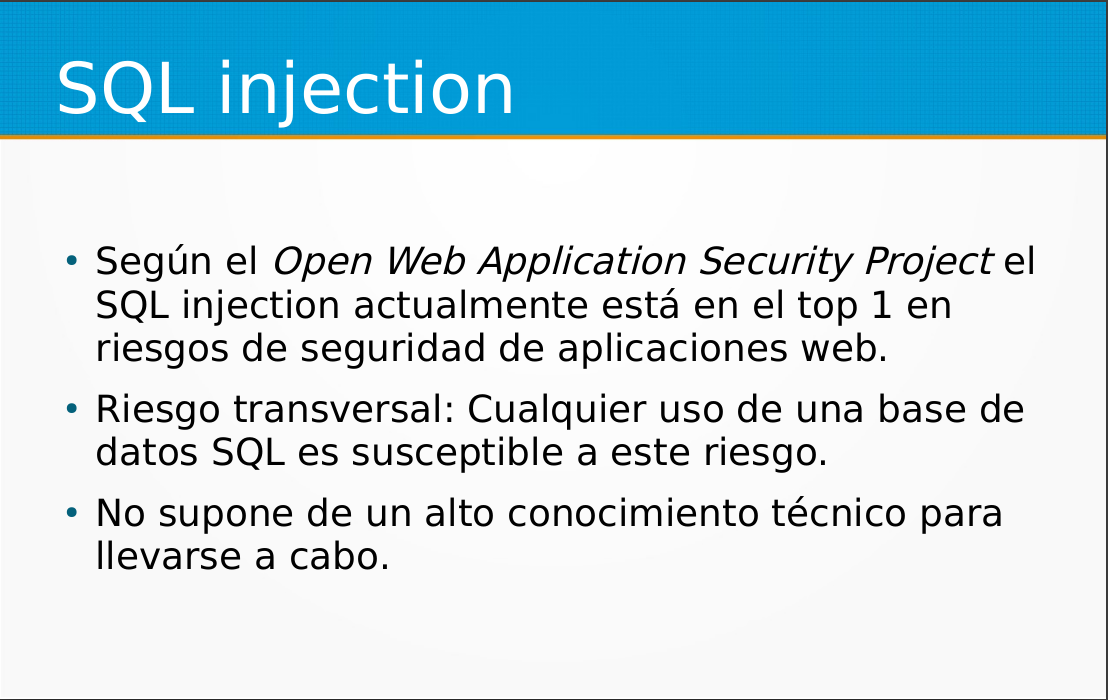
\includegraphics[scale=0.3]{images/1.png}
  \caption{Slide 1}
  \label{fig:1}
\end{figure}
En esta slide primero sentaría las bases del problema a tratar:
\begin{itemize}
\item Qué es una base de datos
\item Cómo la definimos e interactuamos con ella: Lenguaje SQL
\item Cómo la utilizamos en el negocio
\end{itemize}

A continuación explicaría brevemente el concepto de SQL Injection y cómo se puede utilizar para extraer un dato que se supone que no está al alcance de un usuario corriente, quizá acompañado de un ejemplo práctico ya preparado.\\

Acto seguido, explicaría qué es OWASP y cuáles son sus objetivos. Mostraría su top 10 de riesgos de seguridad en aplicaciones web y cómo SQL injection es el número 1 actualmente.\\

Explicaría que todas las bases de datos SQL utilizan las mismas sentencias que permiten la inyección: SELECT, UPDATE, DROP, etc.\\

Finalmente expondría que esas sentencias son conocimiento básico para cualquier tema que trate base de datos y que es sencillo adquirirlo en internet junto con los conocimientos para realizar la inyección e incluso recursos para practicar.\\

\begin{figure}[h!]
  \centering
  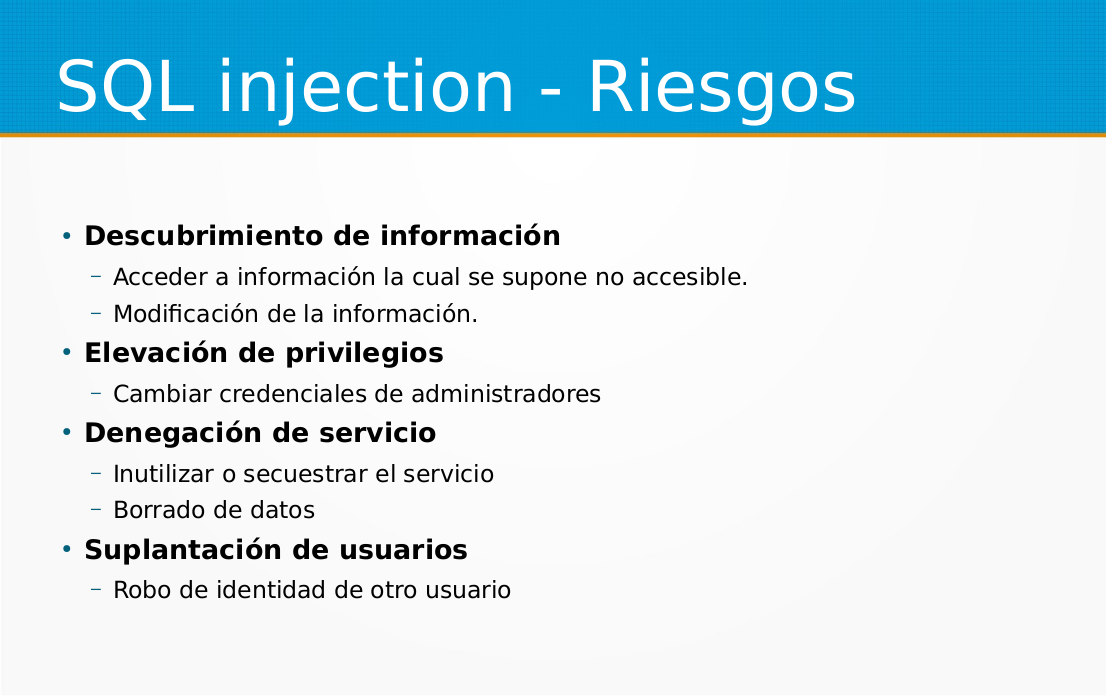
\includegraphics[scale=0.3]{images/2.png}
  \caption{Slide 2}
  \label{fig:2}
\end{figure}

En esta slide enumeraría y detallaría cada uno de los riesgos expuestos: Descubrimiento de  información, elevación de privilegios, denegación de servicios y suplantación de usuarios. Con cada uno expondría un ejemplo de lo que supone para la empresa y cómo algunas tablas y registros se ven expuestas a las inyecciones.\\


\newpage
\begin{figure}[h!]
  \centering
  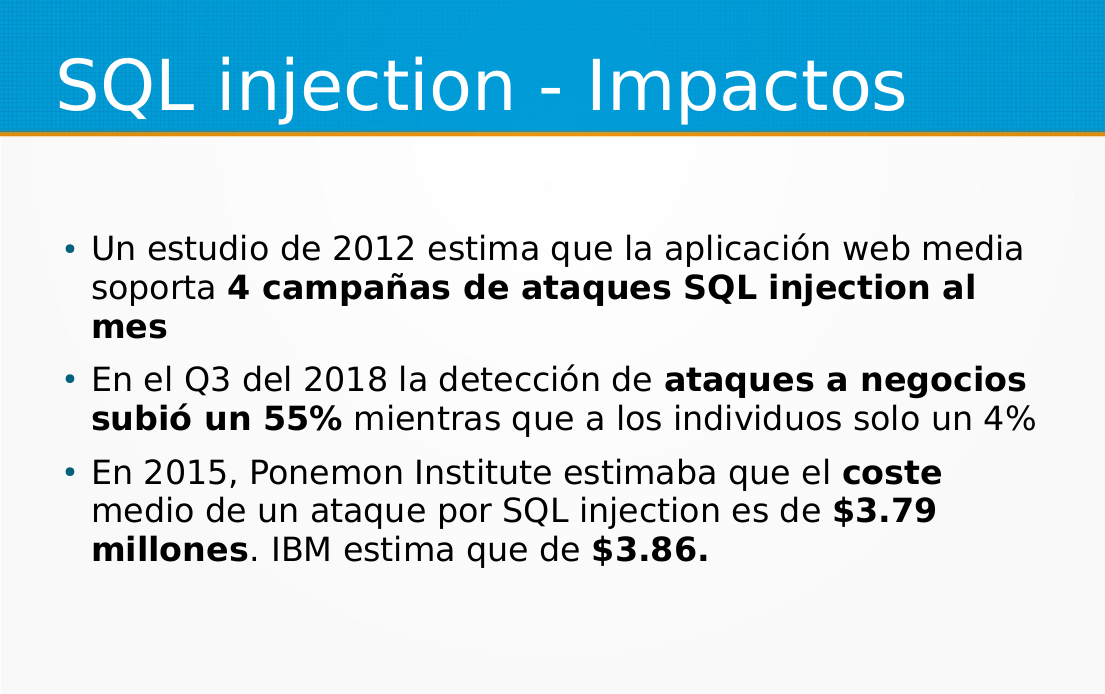
\includegraphics[scale=0.3]{images/3.png}
  \caption{Slide 3}
  \label{fig:3}
\end{figure}

En esta diapositiva hablaría principalmente de algunas cifras calculadas por diferentes estudios sobre los costes que supone este riesgo y los compararía con los costes que supone hacer auditorías y preveer estos fallos de diseño al principio del desarrollo de los proyectos.\\
Acompañaría con ejemplos de otras empresas que se han visto sometidas a estos ataques y lo que ha supuesto tanto para la empresa a nivel económico y legal, como para sus usuarios así como para su imagen corporativa.

\subsection{}
La OWASP proporciona una pequeña guía con conjunto de técnicas sencillas de prevención a vulnerabilidades de SQL injection \cite{sqliprev} para prácticamente todo tipo de lenguaje de programación y todo tipo de base de datos. Las ténicas que se proponen son:

\begin{enumerate}
\item \textbf{Sentencias preparadas con queries parametrizadas}: Se trata de un estilo de codificación que permite a la base de datos distinguir el código de los datos independientemente del input. Consiste en definir primero todas las queries y luego pasarle los parámetros. Muchos lenguajes implementan sus propios métodos para utilizar esta ténica.
\item \textbf{Procedimientos almacenados (Stored Procedures).}
\item \textbf{Listas blancas y validación de inputs}: Existen partes en una query donde no es apropiado el uso de parámetros en la misma como el nombre de tablas o los indicadores de orden (ASC o DESC), lo ideal es que estos datos vengan establecidos por el código de la aplicación y no del input. En estas situaciones es mejor rediseñar la query o validar el input del usuario.
\item \textbf{Escapar todo el input suministrado por usuarios}.
\end{enumerate}

Se pueden implementar algunas defensas adicionales:

\begin{itemize}
\item Privilegios mínimos: Consiste en minimizar los privilegios asignados a cada cuenta que tiene acceso a la base datos. No asignar privilegios de administración.
\item Auditorías de seguridad regulares
\item Revisar la política de seguridad regularmente
\item Tratamiento de errores de la aplicación: Consiste en no dar demasiada información a los usuarios en caso de error, dar la mínima información necesaria para resolver el error para que no haya filtrado de información.
\item Vigilar accesos sospechosos: Se puede restringir el acceso a peticiones que sigan una serie de patrones sospechosos como accesos regulares muy seguidos o con input considerado peligroso.
\end{itemize}

Finalmente, como directriz del diseño de aplicaciones seguras es aplicar el sentido común y estar al día en las nuevas vulnerabilidades que se van descubriendo así como intentar en la medida de lo posible arreglar el software que se sabe que tenga una vulnerabilidad registrada.

\subsection{}
Para detectar ataques de SQLi existen ciertas medidas y herramientas que filtran el tráfico entrante a la aplicación en busca de sentencias de código maliciosas que pudieran suponer un riesgo, como el filtrado de parámetros de entrada.
El filtrado de parámetros de entrada consiste en tratar la entrada de datos en búsqueda SQL injection, en caso de que dicho filtrado encontrara una sentencia de SQLi se podría considerar que se ha detectado un ataque.\\

Se pueden utilizar sistemas de detección de intrusos (IDS) a medida para aplicaciones web llamados Web Application Firewalls. Estos firewall son aplicaciones que se instalan en servidor para controlar las peticiones malintencionadas que podrían dar lugar a un posible ataque.\\

Se pone la aplicación detrás de este firewall y cada vez que se detecte una petición malintencionada se registra y se da el aviso de intento de ataque y se guarda la información relevante en los logs.

\subsection{}
Suponiendo que en la empresa no existe una política de seguridad definida para estos casos y no haya unas directrices claras de lo que hay que hacer, propondría lo siguiente:\\

Una vez se ha producido y reconocido un ataque primero hay que hacer una evaluación de los daños: qué datos se han visto afectados, qué usuarios, tanto clientes como trabajadores, se han visto afectados por el ataque, el alcance de todo el ataque, etc.\\

El segundo paso sería informar a los afectados siguiendo la normativa vigente y en qué medida se han visto afectados sus datos en los sitemas.\\
En caso de que haya habido un ataque destructivo intentaría reestablecer los datos afectados a un punto anterior mediante el uso de backups o con la colaboración de los usuarios afectados.\\
Además, haría una evaluación de los costes de las pérdidas de las hubiera, esto será importante en un punto posterior.\\

A continuación, evaluaría cómo se ha efectuado el ataque, de qué forma han conseguido vulnerar los sistemas de seguridad (si los hay) y cómo han conseguido la sustracción de información.\\
Una vez hecho esto, estamos en disposición de hacer una evaluación de lo que hay que hacer para mitigar el fallo de seguridad y que no vuelva a ocurrir.\\

Haría una estimación del coste que supone aplicar las nuevas medidas para subsanar el fallo de seguridad y lo compararía con el coste del ataque calculado anteriormente. En este punto nos encontramos con dos posibilidades:\\
\begin{enumerate}
\item Que el coste de mitigación sea mucho mayor que el del ataque, en cuyo caso es posible que a los directivos de la empresa no les interese seguir adelante con el plan
\item Que el el coste de mitigación sea mucho menor o cercano al del ataque y a la proyección de ataques similares en el futuro, en cuyo caso los directivos de la empresa pueden estar de acuerdo en invertir para subsanar los errores.
\end{enumerate}

En el segundo caso se dispondrían los recursos y personas necesarias de la empresa para el desarrollo que mitigue las brechas de seguridad y que no vuelva a ocurrir un ataque similar.\\

En ambos casos se debería actualizar la política de seguridad siguiendo las directrices nuevamente establecidas y añadir lo que se ha aprendido al conjunto de conocimientos de la empresa.

\newpage
\begin{thebibliography}{9}

\bibitem{gdpr1}
	\textbf{What does the General Data Protection Regulation (GDPR) govern?}\\
	European comission [Consultado el 20 de diciembre de 2020]\\
	\url{https://ec.europa.eu/info/law/law-topic/data-protection/reform/what-does-general-data-protection-regulation-gdpr-govern_en}

\bibitem{gdpr2}
	\textbf{¿Quién está obligado a cumplir con el RGPD?}\\
	Emprendepyme.net - Veronica Ruiz 28 de mayo de 2018 [Consultado el 22 de diciembre de 2020]\\
	\url{https://www.emprendepyme.net/quien-esta-obligado-a-cumplir-con-el-rgpd.html}

\bibitem{gdpr}
	\textbf{Reform of EU data protection rules}\\
	European comission [Consultado el 20 de diciembre de 2020]\\
	\url{https://eur-lex.europa.eu/legal-content/EN/TXT/?uri=CELEX:02016R0679-20160504}

\bibitem{rgpd}
	\textbf{Reglamento General de Protección de Datos} [Consultado el 22 de diciembre de 2020]\\
	\url{https://rgpd.es/}

\bibitem{funciones}
	\textbf{Base de conocimientos RGPD UE}\\
	Funciones clave definidas en el RGPD de la UE - Punit Bhatia [Consultado el 24 de diciembre de 2020]\\
	\url{https://advisera.com/eugdpracademy/es/knowledgebase/funciones-clave-definidas-en-el-rgpd-de-la-ue/}

\bibitem{elastic1}
	\textbf{El corazón del Elastic Stack, gratuito y abierto}\\
	Elasticsearch [Consultado el 15 de diciembre de 2020]\\
	\url{https://www.elastic.co/es/elasticsearch/}

\bibitem{CVE-2020-7020}
	\textbf{CVE-2020-7020}\\
	CVE Mitre [Consultado el 15 de diciembre de 2020]\\
	\url{https://cve.mitre.org/cgi-bin/cvename.cgi?name=CVE-2020-7020}

\bibitem{CVE-2020-7019}
	\textbf{CVE-2020-7019}\\
	CVE Mitre [Consultado el 15 de diciembre de 2020]\\
	\url{https://cve.mitre.org/cgi-bin/cvename.cgi?name=CVE-2020-7019}

\bibitem{CVE-2020-7014}
	\textbf{CVE-2020-7014}\\
	CVE Mitre [Consultado el 15 de diciembre de 2020]\\
	\url{https://cve.mitre.org/cgi-bin/cvename.cgi?name=CVE-2020-7014}

\bibitem{elastic}
	\textbf{Consejos para asegurar los clusters de Elasticsearch de forma gratuita con encripción, usuarios y más}\\
	Josh Bressers - 4 de Junio de 2019  [Consultado el 15 de diciembre de 2020]\\
	\url{https://www.elastic.co/es/blog/tips-to-secure-elasticsearch-clusters-for-free-with-encryption-users-and-more}

\bibitem{privileges}
	\textbf{Security Privileges}\\
	Elasticsearch [Consultado el 15 de diciembre de 2020]\\
	\url{https://www.elastic.co/guide/en/elasticsearch/reference/7.1/security-privileges.html}
	
\bibitem{painless}
	\textbf{Painless scripting language}\\
	Elasticsearch [Consultado el 15 de diciembre de 2020]\\
	\url{https://www.elastic.co/guide/en/elasticsearch/reference/7.1/modules-scripting-painless.html}
	
\bibitem{scripting}
	\textbf{Scripting security}\\
	Elasticsearch [Consultado el 15 de diciembre de 2020]\\
	\url{https://www.elastic.co/guide/en/elasticsearch/reference/7.1/modules-scripting-security.html}

\bibitem{ccncert}	  	
	\textbf{Vulnerabilidades en Oracle}\\
	CCN-CERT AV 74/20 [Consultado el 20 de diciembre de 2020]\\
	\url{https://www.ccn-cert.cni.es/seguridad-al-dia/avisos-ccn-cert/10615-ccn-cert-av-74-20-vulnerabilidades-en-oracle.html}

\bibitem{CVE-2019-12900}
	\textbf{CVE-2019-12900}\\
	National Vulnerability Database [Consultado el 20 de diciembre de 2020]\\
	\url{https://nvd.nist.gov/vuln/detail/CVE-2019-12900}

\bibitem{CVE-2020-14734}
	\textbf{CVE-2020-14734}\\
	National Vulnerability Database [Consultado el 20 de diciembre de 2020]\\
	\url{https://nvd.nist.gov/vuln/detail/CVE-2020-14734}

\bibitem{CVE-2020-14735}
	\textbf{CVE-2020-14735}\\
	National Vulnerability Database [Consultado el 20 de diciembre de 2020]\\
	\url{https://nvd.nist.gov/vuln/detail/CVE-2020-14735}
	
\bibitem{sqliprev}
	\textbf{SQL Injection Prevention Cheat Sheet}\\
	OWASP [Consutlado el 20 de diciembre de 2020]\\
	\url{https://cheatsheetseries.owasp.org/cheatsheets/SQL_Injection_Prevention_Cheat_Sheet.html}

\end{thebibliography}

\end{document}